\documentclass[a4paper,11pt]{report}
\usepackage[utf8x]{inputenc}
\usepackage{fullpage}
\usepackage[hyphens]{url}
%\usepackage{hyperref} %this messes up the line breaks of url
\usepackage{xspace}
\usepackage{listings}
\usepackage{graphicx}

% Title Page
\title{{CompLACS} Quadrotors Simulator}
\author{Renzo De Nardi,\\University College London\\\texttt{rdenardi@cs.ucl.ac.uk}}

\newcommand{\sname}{QRSim\xspace}
\newcommand{\snamettt}{\texttt{QRSim}\xspace}
\newcommand{\webrepo}{\url{http://complacs.cs.ucl.ac.uk/complacs/simulator/qrsim-lastStable.zip}\xspace}

\begin{document}
\maketitle

\begin{abstract}
This document describes the multi-vehicle quadrotor simulator (\sname) developed at UCL to devise and test algorithms for our flock autonomous helicopters, one of the three application platforms of the {CompLACS} project.
This report is divided into two parts, the first describes the logic and the structure of the simulator while the second presents examples of use. 
Technical details about the dynamic models used in the simulator and their implementation are reported in the appendix. 

A companion to this report is the documentation that Matlab can automatically generate from the source code (i.e. using the command \texttt{doc}), the reader is referred to it for all the more specific API details.
\end{abstract}

\tableofcontents

\chapter{Design and Concepts}

\section{Rationale}\label{sec:rationale}
UAVs provide a rich source of control problems some of which (namely the one connected with individual flight attitude control) have been successfully addressed in previous research (\cite{hoffman08quadrotor},\cite{shim03aflight},\cite{bouabdallah07phd} to list a few). The {CompLACS} project focusses instead on the higher level problems of enabling multiple UAVs to achieve a common goal by communicating and cooperating as an autonomous flock. 

A simulator that allows to devise and test algorithms aiming at such high level problems must reliably model the effects that are (at least to a certain extent) common to all platforms (e.g. wind or GPS errors) as well as the interaction between them.
 
At the same time, since the real platform used in this work are already provided with off-the-shelf stabilisation and attitude controllers, the requirement on accurately simulating the very low level dynamic behaviour of the platform can be relaxed.
Both these sets of requirements make \sname substantially different from existing freely available quadrotor simulators. 


One of the objectives of {CompLACS} is to provide a generic interface to specifying learning and control problems, it is therefore important for the tools used in the initial investigation (i.e. the platforms simulators) to not be constrained to a rigid interface. 
For this reason in \sname more than providing a single and rigid interface to the application platform, we decided to build a modular and extensible API so to make it possible to redefine the platform interface with relative ease. 

Defining concrete application scenarios based on the available platforms and simulators is one of the forthcoming deliverable of {CompLACS} (milestones 6.2, 7.2), this document aims at aiding this process by providing clear description of \sname and of its capabilities. 

\section{Concepts}
We start by presenting the main conceptual blocks that constitute the simulator.

\subsection{Platforms and Environment Objects}\label{sec:platandenv}
Within \sname we make a logical distinction between two types of objects:
\begin{itemize}
\item platforms,
\item environment objects.
\end{itemize}
To the first type belong the description of the quadrotor dynamics but also the models of sensors and other phenomena that are platform specific (e.g. aerodynamic turbulence). The second class comprehends al the phenomena that are not platform specific and have direct or indirect impact on several platforms (e.g. the flight area or the satellite vehicles of the GPS system).
In many ways this distinction is rather natural and in \sname we are simply exploiting it in order to provide a sensible structure to the simulator.

In general the platforms are the only objects that can be controlled by means of actions, of course those might eventually have an indirect effect on the environment. We must underline that this does not impose for any of the two classes to be time invariant; in fact both types of objects might change during the course of a simulation as result of actions or simply as result of the time passing.

To the extent allowed by Matlab we used object-oriented programming concepts in order to map physical objects directly into the corresponding classes. Platforms subclass the abstract class \texttt{Platform} (defined in \texttt{/qrsim/platforms/Platform.m}) and environment objects subclass \texttt{EnvironmentObject} (defined in \texttt{/qrsim/environment}).

\subsection{State}\label{sec:state}

At any point in time the simulator must maintain the state of all the objects taking part in the simulation, this is accomplished with a data structure is defined by a Matlab class called (rather obviously) \texttt{State}.
 
A handle to a object of this type is returned during the initialisation of the simulator and can be used to reference the various objects part of the simulation. For instance the fields \texttt{environment} and \texttt{platforms} store respectively the handles to all the environment objects and to the cell arraay of platforms objects. 
Given such a structure accessing the state of objects is trivial, for instance \texttt{state.platforms{1}.getX()} gives access to the state variables of the first platform, while \texttt{state.environment.area.getLimits()} returns the size of the flying area. 

When meaningful, the \texttt{Platform} and \texttt{EnvironmentObject} classes define methods to retrieve the object state (e.g. \texttt{getX()} in the case of a platform), to reset the state to its initial value defined by the task (see section \ref{sec:createtask}) and to set the object state (e.g. \texttt{setX(X)} in the case of a platform)\footnote{In addition to overwriting the object's state these calls also make sure that any other internal variable (e.g. noise model states) is appropriately set.}.

The \texttt{State} structure stores also other important variables:
\begin{itemize}
 \item the simulator time (field \texttt{t}), used to ensure synchronization between all the environment and platforms objects;
 \item the independent pseudo-random number generator streams (field \texttt{rStreams}), used by any of the objects that requires any form of random numbers (e.g. to simulate noise samples);
 \item the simulator time step (field \texttt{DT}), the time granularity with which the simulator time is incremented;
 \item the handle to the 3D graphics visualization (field \texttt{display3d}).
\end{itemize}

\subsection{Steppable}

Since the platforms and environment that we are simulating are representation of physical objects, one simple way to think about their evolution in time is to consider time discretized into steps and to ``step forward'' the object's state at each time step. In the case of a quadrotor for instance, stepping forward is nothing more than integrating the ODE that describe its dynamics, for other objects stepping forward might mean instead triggering an event associated with a specific time.
In our implementation every object that evolves with time is derived from a common class (i.e. \texttt{Steppable}) which defines an abstract \texttt{update()} method and a time step property \texttt{dt}.

The method \texttt{update()} propagates the object's state forward to the current time (field \texttt{t} of the \texttt{State} data structure), the object's field \texttt{dt} specifies with what (time) granularity \texttt{update()} should be called. 

As we will see in section \ref{sec:qrobj}, the \texttt{update()} method is never called directly, instead the  \texttt{Steppable} class exposes the method \texttt{step()} which in turns only calls \texttt{update()} if a time equal to \texttt{dt} has passed since the last update\footnote{To simplify the implementation the time step \texttt{dt} of any object must be a multiple of the simulator time step (\texttt{DT}); in practice this is not a very restrictive assumption.}.

\subsection{Task}

By combining different types of environment objects and platforms \sname allows to define a variety of single and multiple helicopter scenarios as well as many different objectives for the platforms.

The abstract class \texttt{Task} provides a way to derive task objects that specify both a scenario and an activity to be learned; the class defines two main methods \texttt{init()} and \texttt{reward()}:
\begin{itemize}
 \item \texttt{init()} allows the user to define the type of each of the environment objects (i.e. the class name) and of each platform and sensor. Along with the object type, a specification of all the class specific parameters is also needed.
 \item \texttt{reward()} allows for defining an instantaneous reward for the task, this can be used for the purpose of learning. The design of a reward function is very task specific but most often the user will rely on the \texttt{state} data structure in order to compute such a reward.
\end{itemize}

We will present how to create a task in section \ref{sec:createtask}.

\subsection{Other Abstract Classes}

At the aim of making the code easy to extend, the software API defines also several other abstract classes:
\begin{itemize}
\item \texttt{AerodynamicTurbulence}
\item \texttt{Sensors}
\item \texttt{AHARS}
\item \texttt{OrientationEstimator}
\item \texttt{Gyroscope}
\item \texttt{Altimeter}
\item \texttt{Accelerometer}.
Such abstract classes are used very much like software interfaces and allow to configure specific type of sensor through the task object parameters (see section \ref{sec:createtask}), in this way the correct class is loaded at run time.
\end{itemize}

\section{The \sname Object}\label{sec:qrobj}

After a brief introduction of the fundamental building blocks of \sname we can look at how they are used within the main class of the simulator. 

The object \snamettt allows to initialize, set up and control the simulator as a whole. 

\snamettt exposes three main methods:
\begin{itemize}
 \item \texttt{init('task\_name')}, initializes the platforms the environment objects and the task according to what specified by the task \texttt{'task\_name'} (see section \ref{sec:createtask}) and creates the \texttt{state} data structure. This is generally the first command called soon after the creation of the \snamettt object and must be called only once.
 \item \texttt{reset()}, resets the simulator to the initial state specified by the task. This is generally called after a learning episode in order to restore the state of the simulator. 
 \item \texttt{step(U)}, steps forward in time all the environment objects and all the platforms . This command accepts a matrix of control inputs \texttt{U} (i.e. one column array for each platform) and calls the \texttt{step()} method for each of the objects. Listing~\ref{lst:step} shows the implementation of the method.

Very simply, first \texttt{obj.state.t} is updated\footnote{This is the only statement that updates the simulation time.}, then all the environment object are propagated and only later each of the platform is stepped forward. At this point the new state of the platforms can be accessed as described in section \ref{sec:state}.
 \item \texttt{reward()}, returns the instantaneous reward defined by the current task. This is simply a pass through call to the task \texttt{reward()} method and is meant to be called after stepping the simulator.
\end{itemize}

\begin{lstlisting}[float=ht!bp,caption=\sname step() method,language=Matlab,frame=lines,label=lst:step,numbers=left,basicstyle=\small]
function obj=step(obj,U)
           
  %% update time
  obj.state.t=obj.state.t+obj.state.DT;
                        
  %% step all the common objects
            
  % the space segment of the GPS
  obj.state.environment.gpsspacesegment.step([]);
            
  % the wind
  obj.state.environment.wind.step([]);
            
  %% step all the platforms            
  for i=1:length(obj.state.platforms)
    obj.state.platforms{i}.step(U(:,i));
  end
end
\end{lstlisting}


\chapter{Installation and Use}

\section{Installation}
The simulator is entirely written in Matlab and does not depend on any additional toolbox; the only requirement is a recent version of Matlab (i.e. version number greater  than 7.6; see section \ref{sec:testedos} for details on the configurations tested).

To retrieve the software one can simply clone the git\footnote{The git version control software is available for Linux (usually from the package manager), OSX (http://code.google.com/p/git-osx-installer/) and Windows (http://code.google.com/p/msysgit/)} source code repository\footnote{Please note that currently the git repository is read only.} into a directory of choice:
\begin{verbatim}
$ git clone http://complacs.cs.ucl.ac.uk/git/qrsim.git
$ cd qrsim
$ git checkout -b lastStable
\end{verbatim}
Alternatively, the \texttt{lastStable} tag of the software repository is also available as a zip archive from \webrepo. In this case the archive needs to be downloaded and unpacked into a directory of choice.

Once we have the software in a local directory (let's assume it to be \texttt{\textasciitilde/qrsim}), in order to use it is necessary to add the absolute path to the \texttt{sim} directory to the current Matlab search path. 
This can be done using the menu \textsf{File \textgreater ~Set Path} from the Matlab toolbar. Alternatively this can be done from the Matlab console: after navigating to the local simulator directory (\texttt{\textasciitilde/qrsim} in our example) one can issue the command\footnote{Note that this command depends on the location from which it is executed.} 
\begin{verbatim}
>> addpath([pwd,filesep,'sim']);
\end{verbatim} 

You now have all that is needed to run the basic exampls \texttt{main.m} and \texttt{main10.m}. 
To do so navigate to the \texttt{example} directory (i.e. \texttt{\textasciitilde/qrsim/example}) and then simply run the \texttt{main.m} script.
If \texttt{main.m} fails with the message 
\begin{verbatim}??? Undefined function or variable 'QRSim'\end{verbatim}
the path was not set correctly; use the toolbar menu \textsf{File \textgreater ~Set Path} to confirm that the absolute path of the directory \texttt{sim} was added correctly.

At the aim of improving performance, some of the most computationally expensive functions in the simulator have been written also as MEX function, these can be easily compiled using the function \texttt{mexify('compile')}\footnote{Depending on your system setup you might need to configure the MEX compiler using \texttt{mex -setup}; please refer to the Matlab documentation for more details.}.

\subsection{Tested OS} \label{sec:testedos}

The software was tested succesfully on the following setups :
\begin{itemize}
 \item Ubuntu 11.10 with Matlab R2010b and gcc version 4.6.1\footnote{With gcc 4.6.1 mex compilation warns the user that gcc 4.6.1 is not a supported compiler, in our experience this warning can be safely ignored.}.
 \item Windows XP SP3 with Matlab 2010a.
 \item Windows Server 2008 R2 with Matlab 2011a and Visual Studio 2008.
 \item OSX 10.5 with Matlab 2010a and Xcode gcc version 4.2\footnote{We removed the option \texttt{-isysroot} from the \texttt{CFLAGS} and \texttt{CXXFLAGS} in the file \texttt{mexopts.sh}. For newer versions of Xcode see \url{http://www.mathworks.co.uk/support/solutions/en/data/1-FR6LXJ/}}.
\end{itemize}

\section{Creating a Task}  \label{sec:createtask}

As a first example of use we look at a single platform task which requires to maintain the quadrotor hovering at the position it has when the task starts; the solution requires to adjust continuously controls since the helicopter is affected by time varying wind disturbances. We call this task TaskKeepSpot. 
 
To implement such a task, we start by creating a new class that extends the abstract class \texttt{Task} and implements the \texttt{init()} and \texttt{reward()} methods.

The \texttt{init()} method (see listing \ref{lst:init}) 
\begin{lstlisting}[float=ht!bp,caption=TaskKeepSpot init() method,language=Matlab,frame=lines,label=lst:init,numbers=left,basicstyle=\small]
function taskparams=init(obj)  
 taskparams.DT = 0.02; % Simulator step time in seconds            
 taskparams.seed = 0; % if 0 the seed depends on the system time
            
 %%%%% visualization %%%%%
 % 3D display parameters
 taskparams.display3d.on = 1;
 taskparams.display3d.width = 1000;
 taskparams.display3d.height = 600;            
            
 %%%%% environment %%%%%
 % these need to follow the conventions of axis(), they are in m, Z down
 taskparams.environment.area.limits = [-10 20 -10 10 -20 0];
 taskparams.environment.area.type = 'BoxArea';
            
 % originutmcoords is the location of the RVC (our usual flying site)
 % generally when this is changed gpsspacesegment.orbitfile and 
 % gpsspacesegment.svs need to be changed
 [E N zone h] = lla2utm([51.71190;-0.21052;0]);
 taskparams.environment.area.originutmcoords.E = E;
 taskparams.environment.area.originutmcoords.N = N;
 taskparams.environment.area.originutmcoords.h = h;
 taskparams.environment.area.originutmcoords.zone = zone;
 taskparams.environment.area.graphics.type = 'AreaGraphics';
            
 % GPS - the space segment of the gps system
 taskparams.environment.gpsspacesegment.on = 1; % noiseless gps if 0
 taskparams.environment.gpsspacesegment.dt = 0.2;
 % real satellite orbits from NASA JPL
 taskparams.environment.gpsspacesegment.orbitfile = 'ngs15992_16to17.sp3';
 % simulation start in GPS time, this needs to agree with the sp3 file above, 
 % alternatively it can be set to 0 to have a random initialization 
 taskparams.environment.gpsspacesegment.tStart = 0;             
 % id number of visible satellites, to match the contents of orbitfile
 taskparams.environment.gpsspacesegment.svs=[3,5,6,7,13,16,18,19,20,22,24,29,31];
 % the following model was instead designed to match measurements of real data
 taskparams.environment.gpsspacesegment.type = 'GPSSpaceSegmentGM2';            
 taskparams.environment.gpsspacesegment.PR_BETA2 = 4; % time constant
 taskparams.environment.gpsspacesegment.PR_BETA1 =  1.005; % time constant   
 taskparams.environment.gpsspacesegment.PR_SIGMA = 0.003; % standard deviation            
            
 % Wind - a steady omogeneous wind common to all helicopters
 taskparams.environment.wind.on = 0;
 taskparams.environment.wind.type = 'WindConstMean';
 askparams.environment.wind.direction = degsToRads(45); %mean wind direction
 taskparams.environment.wind.W6 = 0.5;  % velocity at 6m from ground in m/s
            
 %%%%% platforms %%%%%
 % Configuration and initial state for each of the platforms
 taskparams.platforms(1).configfile = 'pelican_config';
 taskparams.platforms(1).X = [0;0;-10;0;0;0];       
end
\end{lstlisting}
returns a data structure that contains general fields like the simulator time step \texttt{taskparams.DT} and the seed of the pseudo-random number generator (\texttt{taskparams.seed}), fields for each of the environment objects (\texttt{taskparams.environment}), and for each of the platforms (\texttt{taskparams.platforms}). The fields depend on the number and type of objects, but by convention we name:
\begin{itemize}
\item \texttt{on}, the flag that allows to enable and disable the object in question,
\item \texttt{dt}, the time step of the object,
\item \texttt{type}, the class name of the object.
\end{itemize}

The number of sensors and parameters present in a platform would make defining several identical platforms quite cumbersome. For this reason all the platform parameters are specified in a single configuration file (see \texttt{'pelican\_config'}); in this way the same file can be used for more than one platform. Nonetheless is still possible to define a different initial position and orientation for each platform using the parameter \texttt{taskparams.platforms(1).X} (see line 51).

Lastly we see the \texttt{taskparams.display3d} parameters which allow to specify if the 3D visualization is active and the size of the window used for its rendering. 

As already explained, a task must also define a reward function. For the TaskKeepSpot task a straightforward reward can be computed subtracting the initial position of the quadrotor from its state vector and taking the square magnitude of the vector obtained (see listing \ref{lst:reward}). 
Such a function gives higher rewards to a policy that maintain the quadrotor close to the starting point but also keeps it level (i.e. \texttt{X(4:6)=0}) and minimizes linear and rotational velocities (i.e. \texttt{X(7:12)=0}).

\begin{lstlisting}[float=ht!bp,caption=TaskKeepSpot reward() method,language=Matlab,frame=lines,label=lst:reward,numbers=left,basicstyle=\small]
function r=reward(obj)
  e = obj.state.platforms{1}.X(1:12);
  e = e(1:3)-obj.state.platforms{1}.params.X(1:3);
  r = - e' * e; 
end
\end{lstlisting}
The complete listing for this task can be found in the file \texttt{TaskKeepSpot.m}.  

\section{Example Main}
To clarify the use of the simulator through the \snamettt object, we shall present a simple example of use\footnote{Source code in the directory \texttt{example}}; namely we will use a manually designed PID controller to achieve the behavior required by the \texttt{TaskKeepSpot} task\footnote{We want to clarify that the PID controller was chosen exclusively for its simplicity, in facts it is a very conservative controller and its performance are suboptimal. This said it might still be useful as a baseline for comparisons.}.

Listing \ref{lst:main} shows the code of this bare bone example. 

\begin{lstlisting}[float=ht!bp,caption=main script,language=Matlab,frame=lines,label=lst:main,numbers=left,basicstyle=\small]

% create simulator object
qrsim = QRSim();

% load task parameters and return hanle to simulator state
state = qrsim.init('TaskKeepSpot');

% create a PID object
pid = WaypointPID(state.DT);

% number of steps we run the simulation for
N = 3000;

% initial position of the helicopter
wp = [state.platforms{1}.getX(1:3)',0];

tstart = tic;

for i=1:N,
    tloop=tic;

    % compute controls based on the ESTIMATED state 
    U = pid.computeU(state.platforms{1}.getEX(),wp);

    % step simulator
    qrsim.step(U);
    
    % get reward
    % qrsim.reward();
    
    % wait so to run in real time
    wait = max(0,state.DT-toc(tloop));
    pause(wait);
end
elapsed = toc(tstart);
\end{lstlisting}
Before anything else we are required to instantiate the \snamettt object, this will make sure that all the functions and classes of the simulator are reachable. Next we load all the task parameters by calling \texttt{qrsim.init()}, such function returns a handle to the simulator state.

The main for loop (see line 17) drives the simulation forward by calling in sequence the PID controller and the \texttt{qrsim.step(U)} method; given the current state of the platform, the PID computes the new control action  \texttt{U} which is then used to step the dynamics forward in time.

A quadrotor requires four control inputs U=[$u_{pt};u_{rl};u_{th};u_{ya}$] respectively pitch roll throttle and yaw.
In hover condition pitch and roll are zero and the throttle is the amount required to counterbalance the gravity force\footnote{With our dynamic model and a mass of $1.68Kg$ the required throttle control is $0.59$} while yaw controls the direction in which the helicopter is pointing.  
Any pitch or roll rotation away from the level attitude will produce a corresponding translational acceleration. To move forward is sufficient a small amount of pitch (negative pitch to be precise), and a roll motion allows to move left and right. 

The PID controller computes the required pitch roll yaw and throttle command proportionally to the current distance between the helicopter and it selected waypoint.

Since we are using a PID controller and no learning is involved, after stepping the simulator we do not make use of the reward returned by the task. In the listing (line 27) we show the call commented out since this is where normally the reward would be computed.

Since the task defines to run the simulation with the 3D visualization, it makes sense to run it in real time, therefore line 30 introduces the necessary pause.  

\begin{figure}
\begin{center}
\label{fig:3d}
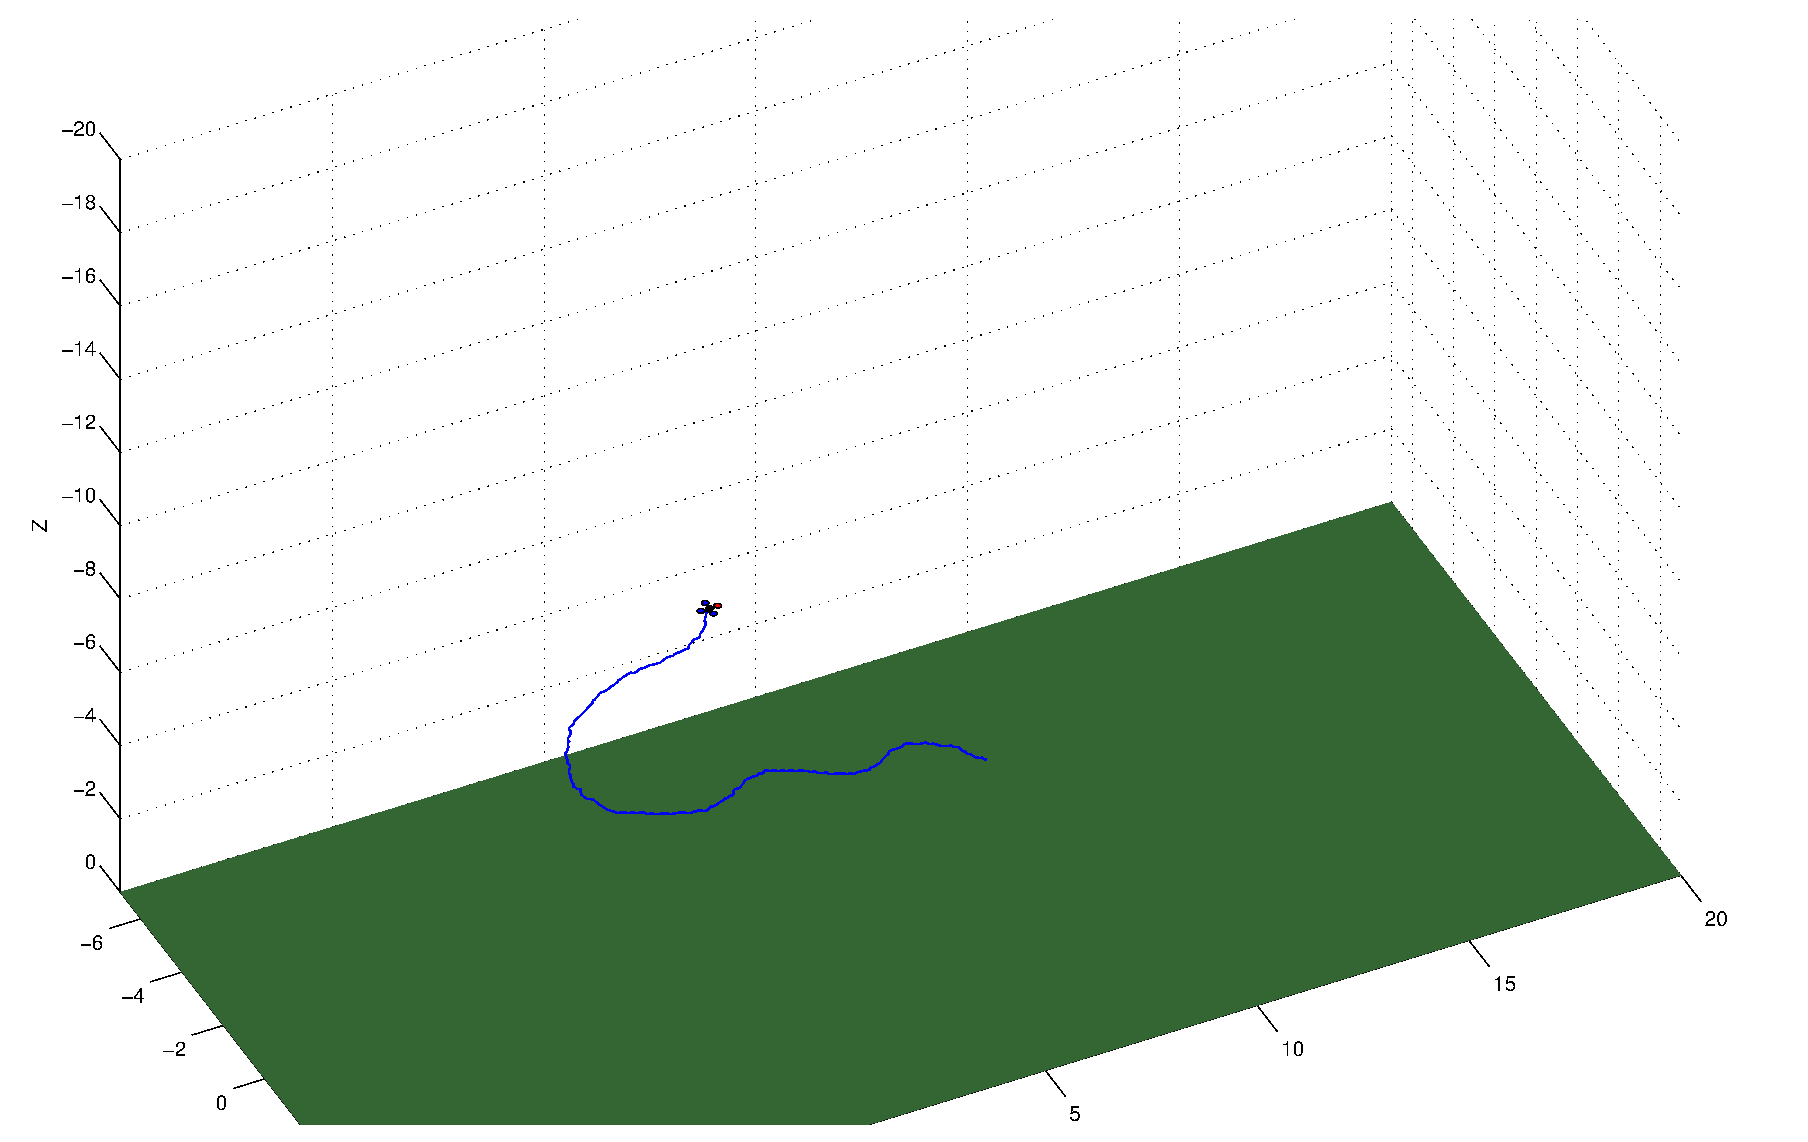
\includegraphics[width=13cm]{./3d.eps}
 \caption{3D visualization}
\end{center}
\end{figure}

Figure \ref{fig:3d} shows a snapshot from the 3D visualization of the simulator where both the platform and its past trajectory are visible.

There is obviously no need to define a specific main script like the one presented above, in certain application for instance it might make more sense to call the \snamettt directly from  a learning algorithm; this is perfectly fine as long as the calls are executed in the same sequence shown in listing \ref{lst:main}.

An additional example called \texttt{main10.m} is also present in the example directory and shows how to generalize the \texttt{TaskKeepSpot} to a group of ten helicopters.

\section{Controllers}

The directory \texttt{/controllers} contain baseline implementations of simple controllers\footnote{We believe these contollers to be qualitatively similar to the ones implemented in the Pelican helicopter, however at present no quantitative comparison has been carried out.} that are often useful in a variety of tasks. Generally such controllers can be used to compute the set of control inputs \texttt{U} given the current state of the platform and a waypoint or velocity that the UAV is meant to reach. 

Currently the following controllers are available:
\begin{itemize}
\item \texttt{WaypointPID} Controller that computes the pitch, roll and throttle input necessary to achieve a desired 3D (NED) velocity in global frame while maintaining a specified heading.
\item \texttt{VelocityPID} Controller that computes the pitch, roll and throttle input necessary to achieve a desired 3D (NED) velocity in global frame while maintaining a specified heading.
\item \texttt{VelocityHeightPID} Controller that computes the pitch and roll input necessary to achieve a desired 2D (NE) velocity in global frame while maintaining a specified altitude and heading.
\item \texttt{HeightHeadingPID} Simple controller that computes the throttle and yaw imput necessary to maintain a specified height and heading. The roll and pitch angle control are left to the user.
\end{itemize}

\section{Multiple Simulations}

Since the implementation of the simulator is completely object oriented, it is possible (and sometimes very useful) to instantiate multiple and completely independent simulations within the same Matlab workspace.  

The script \texttt{/example/multisim.m} shows an example in which one simulator is used to sample control action that are then carried out on the second simulator. 

\section{TCP Interface (Linux)}

We also provide a TCP interface to the quadrotor simulator QRSim so that it functionalities can by easily accessed by a second software. 
The interface is constituted of two parts: a Matlab (Java) server that is responsible for listening to client connection and managing the QRSim simulation and a client library that allows a client to communicate with such server.
Currently the client library is written in C++ for Linux but very similar libraries could be developed easily for other languages\footnote{The data serialization is based on the Google protocol buffers library, so writing a client for any of the languages supported by protocol buffer is pretty straightforward.}.

\subsection{Client}

The client library exposes a series of convenient methods to interact with the Matlab simulator QRSim; we now present them briefly, however we refer to the header file \texttt{QRSimTCPClient.h} and to the QRSim documentation for mare details about the meaning of the parameters.

\begin{itemize}

\item \textbf{\texttt{bool connectTo(string ip, int port)}}\\
  Connects to the Matlab server of QRSim listening at the specified ip address and port. 
  
\item \textbf{\texttt{bool init(string task,vector<vector<double>>\& X,vector<vector<double>>\&\\ \hspace*{55pt} eX,double\& tStep,int\& nUAVs,bool realTime)}}\\
Send to the server the command to initialize the simulator by loading the specified task file; the initial state is returned;

\item \textbf{\texttt{bool reset()}}\\
Sends a reset command to the server, this will cause the simulator to set itself to the initial state defined in the task.

\item \textbf{\texttt{bool disconnect()}}\\
Disconnects from the server without turning off the simulator.

\item \textbf{\texttt{bool quit()}}\\
Disconnects from the server and turns off the simulator.

\item \textbf{\texttt{bool setState(const vector<vector<double>>\& X)}}\\
Send to the server the command to set the UAV noiseless states to the values provided. The state must be within the limits specified in the task.

\item \textbf{\texttt{bool stepWP(double dt,const vector<vector<double>>\& WP,\\ \hspace*{68pt} vector<vector<double>>\& X,vector<vector<double>>\& eX)}}\\
Step forward the simulator giving to each of the UAVs the specified waypoint as input.
The simulator uses a PID in order to reach the specified waypoint, once the waypoint is achieved the UAV will remain stationary at the waypoint.

\item \textbf{\texttt{bool stepVel(double dt, const vector<vector<double>>\& vel,\\ \hspace*{72pt} vector<vector<double>>\& X,vector<vector<double>>\& eX)}}\\
Steps forward the simulator giving to each of the UAVs the specified velocity commands as input.
The simulator uses a PID in order to achieve and maintain the velocity command specified.

\item \textbf{\texttt{bool stepCtrl(double dt, const vector<vector<double>>\& ctrl,\\ \hspace*{80pt} vector<vector<double>>\& X,vector<vector<double>>\& eX)}}\\
Steps forward the simulator giving to each of the UAVs the specified control commands as input.
The input is expressed in terms of angles and throttle command so it is directly passed to the dynamic model of the quadrotors.

\end{itemize}

\subsection{Server}
The server code is constituted by a Matlab function (\texttt{qrsim/tcp/matlab/QRSimTCPServer.m}) that takes care of setting up and executing command in the quadrotor simulator and a Java class (\texttt{qrsim/tcp/java/qrsimsrvcli/QRSimTCPServer.java}) which manages the TCP connection and the data serialization.

In general a user of the client library does not need to modify the server code, but this needs to be compiled\footnote{Google protocol buffer serialization tightly depends on the version of the protocol buffer library so shipping a precompiled server library is not a viable option.} and installed (see section \ref{comp} and \ref{inst}) on the machine that will run the quadrotor simulation.

\subsection{Compilation and Installation}

The current version of the TCP interface only supports Linux\footnote{Currently we only tested the code on Ubuntu 12.04LTS, but (assuming that all the dependencies are satisfied) the code should compile in any other recent Linux distribution.}, in the following we assume to be working on one of such systems.

\subsubsection{Dependencies} 
The C++ client uses Google protocol buffers\footnote{https://developers.google.com/protocol-buffers/} for data serialization and the build process uses CMake\footnote{http://www.cmake.org/}, so both of these tools needs to be available in your Linux machine.

On Ubuntu 12.04 these can be installed as follows:
\begin{verbatim}
$ sudo apt-get install cmake
$ sudo apt-get install libprotoc-dev libprotobuf7 libprotobuf-lite7 libprotobuf-java
\end{verbatim}

\subsubsection{Compilation} \label{comp}
To compile the server and client code cd into \texttt{qrsim/tcp/build} and run:
 \begin{verbatim}
$ cmake ..
$ make
\end{verbatim}
all should compile cleanly.

CMake is smart enough to figure out if you do not have Java installed in your machine in which case only the C++ client library will be compiled.
Note that this is a legitimate scenario since you might be interested in connecting to a remote server which takes care of running QRSim. 

\subsubsection{Installation}\label{inst}
Installing\footnote{The library is installed in \texttt{/usr/local/lib} and the header files in \texttt{/usr/local/include/qrsimtcpclient/}.} the library is nothing different from any usual Linux library compiled from source:

\begin{verbatim}
$ sudo make install
\end{verbatim}

\subsection{Using the Client Library in your C++ code}

Now that the client library is compiled and installed in your system, using it in your custom C++ code is straightforward.
As you commonly do with other shared library installed in your system:
\begin{itemize}
\item include the file \texttt{QRSimTCPClient.h} in you source code to have access to the library methods
\item link against libqrsim \texttt{libqrsimtcpclient.so}.
\end{itemize}
The files \texttt{qrsim/tcp/src/exampleclient.cpp} and \texttt{qrsim/tcp/src/testclient.cpp} provide two small examples of using the client library.

\subsection{Running the Server}\label{run}
The server code runs in Matlab; from the Matlab console cd into the directory \texttt{qrsim/tcp/matlab} and run:
\begin{verbatim}
>> QRSimTCPServer(10000)
\end{verbatim}
where \texttt{10000} is the number of the TCP port you want to use. As the program starts you should see the following message:
\begin{verbatim}
>> QRSimTCPServer(10000)
Waiting for client to connect to this host on port : 10000
\end{verbatim}
indicating that the server is running correctly and is awaiting for connecting from the client.

\subsection{Testing the Interface}

We provide a simple binary to test the TCP interface, after the compilation this should be present in the directory \texttt{qrsim/tcp/bin}.
Once the server is up and running you can run the client as follows:
\begin{verbatim}
$ testclient 127.0.0.1 10000
\end{verbatim}
where \texttt{127.0.0.1} and \texttt{10000} are the IP address and TCP port of the server.
If the tests run successfully you should obtain the following output:
\begin{verbatim}
$ ./testclient 127.0.0.1 10000
QRSIM init test[PASSED]
QRSIM reset test [PASSED]
QRSIM stepWP test [PASSED]
QRSIM stepCtrl test [PASSED]
QRSIM stepVel test [PASSED]
QRSIM disconnect test [PASSED]
QRSIM quit test [PASSED]
\end{verbatim}



\appendix
\chapter{Implementation Details}

This appendix describes the models implemented in \sname in order to replicate a typical quadrotor platform (namely the Ascending Technologies Pelican \cite{asctec2011pelican} in use at UCL) complete of its sensors.
We primarily aim at giving a basic explanation of our implementation choices to the non expert, for more in depth treatment we refer to the publications referred in each of the following sections.

\section{Reference Frame and Symbols}

For convenience we show the body frame of reference used in many of the computation involving the helicopter dynamics (see figure \ref{fig:axes}).
 
The global frame (not shown in the figure) is defined as the local tangent plane to the earth surface at the origin. 
By definition the body and global frame coincide when the quadrotor is at coordinates $(0,0,0)$ and its attitude is zero in all three angles.
\begin{figure}[htbp]
 \begin{center}
 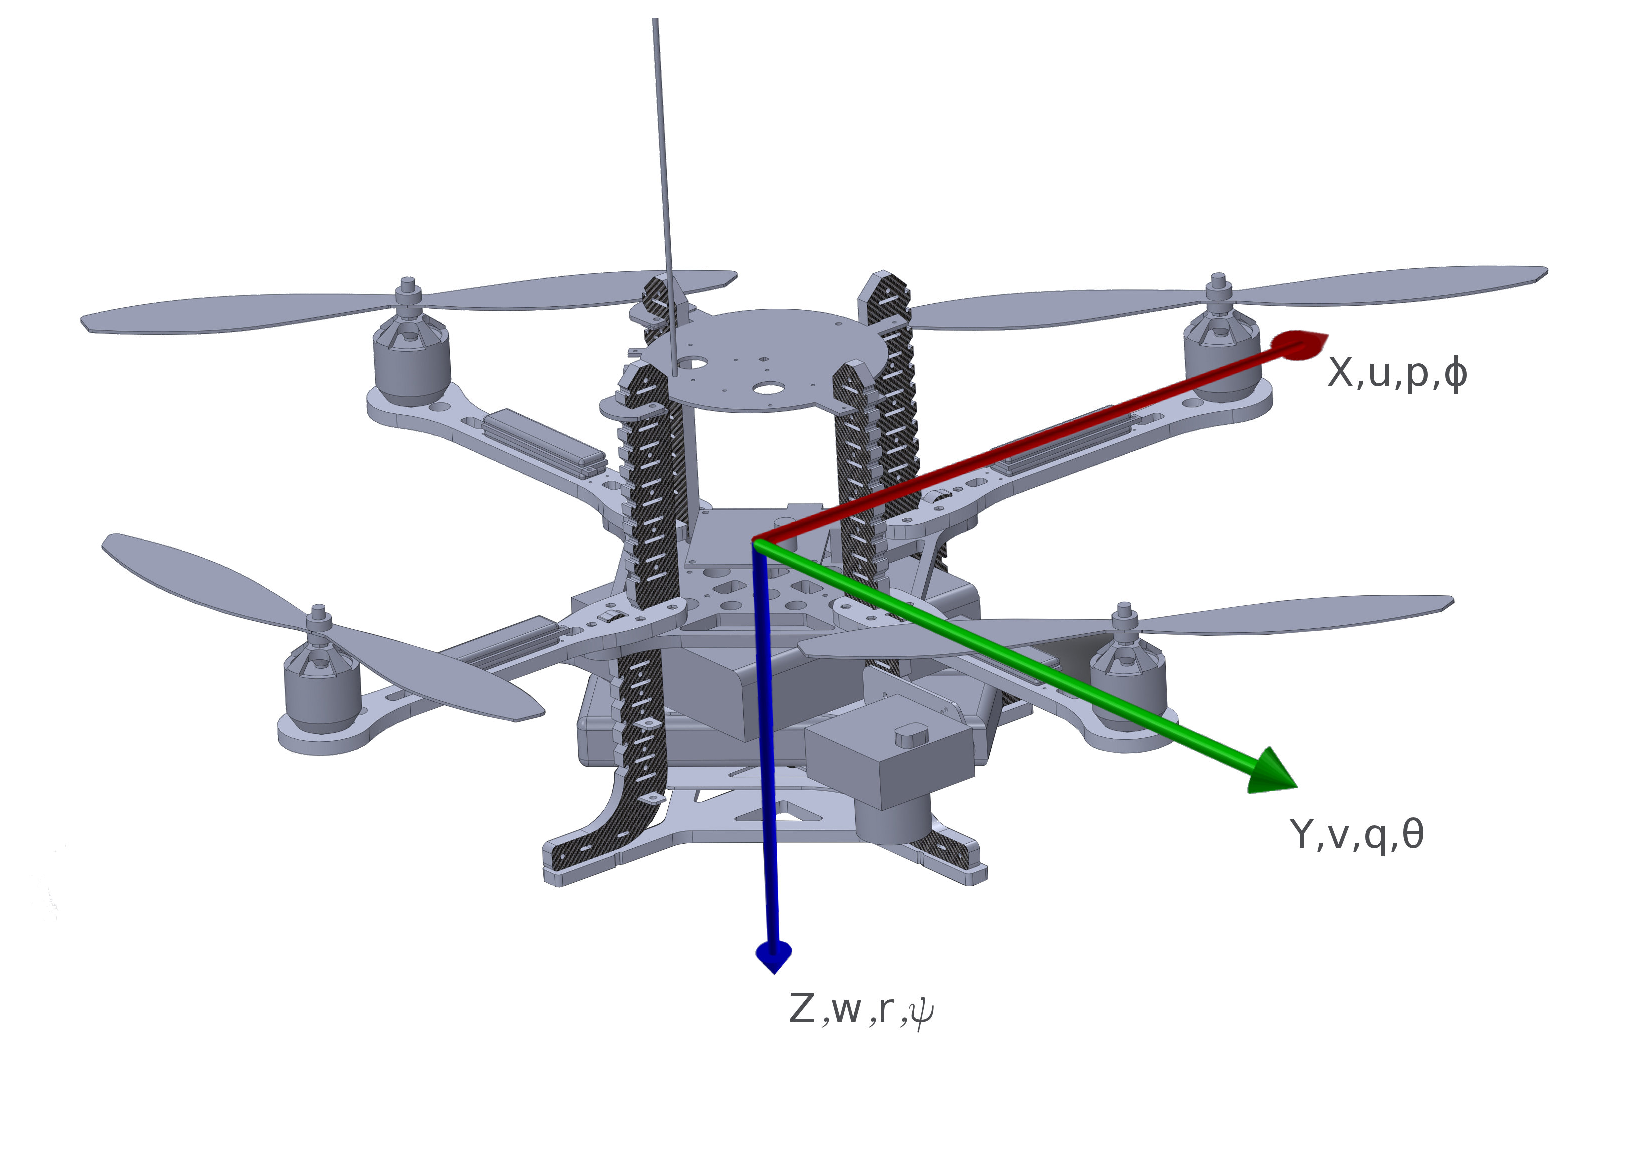
\includegraphics[width=13cm]{./axes.eps}
\caption{Body NED frame of reference and state variables.\label{fig:axes}}
\end{center}
\end{figure} 

We also define first several of the variable that are used in the simulator:
\begin{itemize}

\item \textbf{True platform state} X = [$p_x;p_y;p_z;\phi;\theta;\psi;u;v;w;p;q;r;F_{th}$]

\begin{tabular}{lll}
    $p_x$ & x position (NED coordinates)                            & $m$\\
    $p_y$ & y position (NED coordinates)                            & $m$\\
    $p_z$ & z position (NED coordinates)                            & $m$\\
   $\phi$ & roll attitude in Euler angles right-hand ZYX convention & $rad$\\
 $\theta$ & pitch attitude in Euler angles right-hand ZYX convention & $rad$\\
   $\psi$ & yaw attitude in Euler angles right-hand ZYX convention  & $rad$\\
     $u$  & linear velocity along x body axis                       & $m/s$\\
     $v$  & linear velocity along y body axis                       & $m/s$\\
     $w$  & linear velocity along z body axis                       & $m/s$\\
     $p$  & rotational velocity around x body axis                  & $rad/s$\\ 
     $q$  & rotational velocity around y body axis                  & $rad/s$\\ 
     $r$  & rotational velocity around z body axis                  & $rad/s$\\ 
 $F_{th}$ & thrust force                                            & $N$
\end{tabular} 
\\

\item  \textbf{Estimated platform state} eX = [$\tilde{p}_x;\tilde{p}_y;\tilde{p}_z;\tilde{\phi};\tilde{\theta};\tilde{\psi};0;0;0;\tilde{p};\tilde{q};\tilde{r};0;\tilde{a}_x;\tilde{a}_y;\tilde{a}_z;h;\dot{p}_x;\dot{p}_y;\dot{h}$]

\begin{tabular}{lll}
    $\tilde{p}_x$ & x position estimate from GPS (NED coordinates)            & $m$\\
    $\tilde{p}_y$ & y position estimate from GPS (NED coordinates)            & $m$\\
    $\tilde{p}_z$ & z position estimate from GPS (NED coordinates)            & $m$\\
   $\tilde{\phi}$ & roll attitude in Euler angles right-hand ZYX convention & $rad$\\
 $\tilde{\theta}$ & pitch attitude in Euler angles right-hand ZYX convention& $rad$\\
   $\tilde{\psi}$ & yaw attitude in Euler angles right-hand ZYX convention  & $rad$\\
     $\tilde{p}$  & rotational velocity around x body axis from gyro                 & $rad/s$\\ 
     $\tilde{q}$  & rotational velocity around y body axis from gyro                 & $rad/s$\\ 
     $\tilde{r}$  & rotational velocity around z body axis from gyro                & $rad/s$\\
    $\tilde{a}_x$ & linear acceleration in x body axis from accelerometer            & $m/s^2$\\
    $\tilde{a}_y$ & linear acceleration in y body axis from accelerometer             & $m/s^2$\\
    $\tilde{a}_z$ & linear acceleration in z body axis from accelerometer             & $m/s^2$\\
   $h$& altitude\footnotemark  from altimeter NED & $m$\\
    $\dot{p}_x$ & x velocity from GPS (NED coordinates)            & $m/s$\\
    $\dot{p}_y$ & y velocity from GPS (NED coordinates)            & $m/s$\\
   $\dot{h}$    & altitude rate from altimeter NED                   & $m/s$\\
\end{tabular} 
\footnotetext{It is worth noting that $h=-p_z$ therefore as result of a climb maneuver $h$ increases but $p_z$ decreases.}
\\

\item \textbf{Platform controls} U = [$u_{pt};u_{rl};u_{th};u_{ya};V_b$]

\begin{tabular}{lll}
    $u_{pt}$ & pitch command & $rad$\\
    $u_{rl}$ & roll command & $rad$\\
    $u_{th}$ & throttle command & unitless \\
    $u_{ya}$ & yaw command & $rad/s$\\
    $V_b$  & battery voltage & V
\end{tabular}
\\
 
\end{itemize}


\section{Quadrotor Dynamic Model}

Several dynamic models of quadrotor helicopters based on first principles have been published in the literature (\cite{bouabdallah07phd}, \cite{balas07modelling}, \cite{hoffmann07quadrotor}), such examples consider the forces and moments acting on the helicopter in order to obtain the rotational and translational dynamics.

These type of models replicate only the ``mechanics'' and the aerodynamics of the flying machine but do not include the action of the low level control system necessary to stabilise the rotational dynamics. Since the manufacturer of our quadrotor does not make public the design of the stabilization system, simulating it is not a straightforward task. 

Given that the low level dynamics of the quadrotor is not our primary interest (as explained in section \ref{sec:rationale}), for the rotational dynamics we prefer to use an equivalent  model that replicates directly the combined effect of both the quadrotor and of its controller.
We learn the parameter of such a model directly from flight data in order to match as accurately as possible the characteristics of our flight machine.

\subsubsection{Rotational Dynamics}
For the translational dynamics we use a more standard model that consider the forces acting on the center of mass of the flight machine but we learn from data the relationship between the throttle control input and the generated thrust force. This is known to be very much dependent on the type of motors and propellers, learning it ensures we tch the characteristics of our platform.

In the case of the pitch and roll motion the Pelican platform accepts as control input the angles that the platform should maintain ($u_{pt}$ and $u_{rl}$ respectively); our model needs to map such controls into the rate of change of the corresponding rotational velocities $q$ and $p$. 
From flight tests data we deemed that a second order model can provide a good representation of the dynamic response of the state variable $\theta$ and $\phi$ to changes in control. It was also evident that the low level controller drives the propellers so to limit the maximum rotational velocity (a common precaution that ensure to not exceed the sensing and/or control envelope). 

We encoded these findings in equations \ref{eqn:p} and \ref{eqn:q} where $K_{pq0}$, $K_{pq1}$ and $K_{pq2}$ are constant factors that are obtained from flight data while $p_{max}=q_{max}$ are derived from the platform firmware settings.
\begin{equation}\label{eqn:p}
\dot{p}  =  \left\{ \begin{array}{l l} K_{pq1} (K_{pq0} u_{rl} - \phi) + p K_{pq2} & |p|<p_{max} \\ 0  & |p|\geq p_{max} \end{array} \right .\\
\end{equation}
\begin{equation}\label{eqn:q}
\dot{q}  =  \left\{ \begin{array}{l l} K_{pq1} (K_{pq0} u_{pt} - \phi) + q K_{pq2} & |q|<q_{max} \\ 0  & |q|\geq q_{max} \end{array} \right .\\
\end{equation}
Perhaps quite obviously the same parameters are used for the pitch and roll dynamics since the platform is symmetric. 

In the case of the yaw motion the control input to the pelican platform takes the for of the desired yaw speed $u_{ya}$. Even in this case a second order model provides a good fit to the flight data and leads to equation \ref{eqn:r}. 
\begin{equation}\label{eqn:r}
\dot{r} = K_{r0} u_{ya} + r K_{r1}.
\end{equation}
Again the constants were obtained from flight data. 

A Gaussian white noise component is added to each of the angular velocity derivatives in order to account for those effects that are not captured by the model. 

\subsubsection{Translational Dynamics}

In the case of the translational dynamics the first relationship to capture is the one between the throttle control input ($u_{th}$) and the thrust force ($F_{th}$) experienced by the quadrotor. 
Through a series of static tests emerged that the relationship between throttle and thrust can be represented by a second order polynomial: 
\begin{equation}
F_T = C_{th0} + C_{th1} u_{th} + C_{th2} u^2_{th} \label{eqn:ft}
\end{equation}
 this is a typical result (\cite{denardi2010phd},\cite{hoffmann07quadrotor}) in accordance with basic lift theory which predicts a lift proportional to the square of the blades speed.
Full throttle tests also evidenced that the maximum thrust is proportional to the current battery voltage ($V_b$) and decreases as the battery depletes: 
\begin{equation}
F_M = C_{vb0}+C_{vb1} V_b \label{eqn:fm}.
\end{equation}

As expected due to inertia and drag effects, dynamic tests showed that the thrust can not change instantaneously, but instead it changes at a constant rate\footnote{We believe that this is due to the speed control loop present in the electronic speed controllers governing the motors.} $\tau_1$. Exception to this are very slow speed ranges for which behaviour compatible with a first order system is exhibited instead. Combining this dynamic behaviour with the maximum thrust defined by the lowest between (\ref{eqn:ft}) and (\ref{eqn:ft}) we obtain:
\begin{equation}
\dot{F}_{th}=\left\{ \begin{array}{l l} -\tau_1 & \max(F_T,F_M)<F_{th} \\ \tau_1  & \max(F_T,F_M)\leq F_{th}. \end{array} \right .\\
\end{equation}

Given $F_{th}$, the gravity force in body coordinates $g_b$ and the wind velocity in body coordinates $[u_w,v_w,w_w]$, the resulting accelerations in body coordinates can be computed as:
\begin{eqnarray}
\dot{u} &=& -q w + r v + g_{b_x} + K_{uv}(u-u_w)\label{eqn:u}\\
\dot{v} &=& -r u + p w + g_{b_y} + K_{uv}(v-v_w)\\
\dot{w} & =& -p v + q u + g_{b_z} - \frac{F_{th}}{m} + K_w (w-w_w). \label{eqn:w}
\end{eqnarray}
Where $m$ is the mass of the quadrotor and the the terms $K_{uv}(u-u_w)$,$K_{uv}(v-v_w)$ and $K_w(w-w_w)$ are the effects of the aerodynamic drag. The first two terms on the right hand side of the equations are needed to take into account the fact that the linear velocities $u,v,w$ are expressed in a rotating frame. 
 
Equations (\ref{eqn:p})-(\ref{eqn:r}) and (\ref{eqn:u})-(\ref{eqn:w}) provide the state update equations which are numerically integrated in order to simulate the time evolution of the state variables.

Similarly to the rotational dynamics even for the translational velocity derivatives we consider an additive Gaussian white noise component in order to account for those effects that are not captured by the model. 

The interested reader can find the implementation of the model presented in this section in the file \texttt{pelicanODE.m}.  

\section{Sensors}

On board a real quadrotor platform a series of sensors allows to produce an estimate of the variables that are needed to control and stabilize the helicopter.
A standard suite of sensors (e.g. the ones present on a Pelican) contains a try-axial accelerometer, a set of three gyros, a set of three magnetometers, a pressure sensor and a GPS receiver.

Roughly speaking gyros, accelerometers and magnetometers are combined to estimate the platform attitude (i.e. the angles $\tilde{\phi},\tilde{\theta},\tilde{\psi}$), the GPS is used to determine the position coordinates $\tilde{p}_x$ and $\tilde{p}_y$ and their rate of change $\dot{p}_x$ and $\dot{p}_y$, and the pressure sensor (combined with the accelerometer) provides altitude ($h$) 
and its rate of change ($\dot{h}$).


\subsection{Barometric Altimeter}

Pressure base altimeter constitutes a light weight and economical way of recovering the altitude of a flying machine. Their precision can reach the order of decimeters making them more accurate than a GPS receiver especially when coupled with other sensors. 

The main drawback of an altimeter based on air pressure is that the air pressure tends to change slowly with time due to meteorological effects.  Its noise process is therefore time correlated. Obviously the measured pressure is also affected by the local air turbulence (from the propellers).
Following \cite{stanley1991akalman} and \cite{seo2004position} we model the altimeter measurements as follows:
\begin{eqnarray}
      h&=&-p_z+b_h+\nu_{h_m}  \\
       \dot{b}&=&-\frac{1}{\tau_b}b+\nu_{h_c}
\end{eqnarray}
where $h$ is the of the altimeter, $-p_z$ is true altitude, $b$ is the bias noise which is modelled as first order Gauss-Markov process driven by the white Gaussian noise $\nu_{h_c}$ and $\nu_{h_m}$ is white Gaussian measurement noise. $\tau_b$ is the time constant of the Gauss-Markov process and allows for adjusting the time scale over which the correlation is expressed.
It is worth noting that $-p_z$ is due to our choice of following the aeronautic convention and adopting a NED body frame.

The interested reader can find the implementation of the model presented in this section in the file \texttt{AltimeterGM.m}.  


\subsection{Orientation Estimator}

The orientation of the flying machine is generally estimated on-board using primarily the input from gyros accelerometers and magnetometers, but in some cases might also include  other sensors (i.e. the GPS and barometer). Since all these sensors are combined using an estimator (e.g. a Kalman filter), designing a noise model for the orientation measurement that correctly takes into account the estimation effects is all but trivial. In our case matters are further complicated by the fact that the manufacturer does not make available any clear information about the attitude estimator.
 
Pragmatically we decide to go for a much simpler noise model that attempts to capture the main characteristic of the errors in the estimated attitude. 
Since the primary component of the estimated attitude is the integration of the gyros readings, the orientation noise tends to be correlated due to uncorrected gyro bias errors. 
Additional correlation might be introduced also during high acceleration manoeuvres due to the simplification often adopted in the mechanization equation of the estimator process model.
Errors are mitigated by the use of acceleration and magnetometer measurements which allow to estimate and compensate for such biases.

To replicate such behaviour of reverting back to zero, we choose to model the noise on each each of the three estimated angles a zero mean Ornstein–Uhlenbeck process. This allow to replicate the desired time correlation of the attitude estimates while still being a simple model. The resulting noise model is the following:
\begin{eqnarray}
  \tilde{\phi} &=& \phi + b_\phi\\
  \tilde{\theta} &=& \theta + b_\theta\\
  \tilde{\psi} &=& \psi + b_\psi \\
  \dot{b}_\phi &= &  - \lambda_\phi b_\phi + \nu_{b_\phi}\\
  \dot{b}_\theta &= &  - \lambda_\theta b_\theta + \nu_{b_\theta}\\
  \dot{b}_\psi &= &  - \lambda_\psi b_\psi + \nu_{b_\psi}
\end{eqnarray}
where $\lambda_\phi,\lambda_\theta,\lambda_\psi$ are mean reversion speeds and  $\nu_{b_\phi},\nu_{b_\theta},\nu_{b_\psi}$ are white Gaussian noises.

The interested reader can find the implementation of the model presented in this section in the file \texttt{OrientationEstimatorGM.m}. 

\subsection{Accelerometer and Gyroscope}

Several authors have studied the types of errors that commonly affects accelerometers and gyros (\cite{han2011quantization}\cite{hou2003inertial}) and very accurate, albeit complex, representation of such noise models have been standardised \cite{ieee2006standard}. However since in our platform the low level stabilization is performed on board and is not of interest for the type of activity considered in CompLACS, such type of models are not justified by our requirements. 
At this stage we preferred to go for a simpler model that considers only the main white noise component of the standardized model. The modular nature of the simulator will allow to easily upgrade to a more complex noise model if this is deemed necessary.

For both accelerometer and gyros reading (respectively $[\tilde{a}_x;\tilde{a}_y;\tilde{a}_z]$ and $[\tilde{p};\tilde{q};\tilde{r}]$) the noise is considered additive:
\begin{eqnarray}
  \tilde{p} &=& p + \nu_p\\
  \tilde{q} &=& q + \nu_q\\
  \tilde{r} &=& r + \nu_r
\end{eqnarray}
\begin{eqnarray}
  \tilde{a}_x &=& a_x + \nu_x\\
  \tilde{a}_y &=& a_y + \nu_y\\
  \tilde{a}_z &=& a_z + \nu_z
\end{eqnarray}
where  $\nu_p,\nu_q,\nu_r,\nu_x,\nu_y,\nu_z$ are white Gaussian processes.

The interested reader can find the implementation of the model presented in this section in the file \texttt{AccelerometerG.m} and \texttt{GyroscopeG.m}.  

\subsection{GPS Model}

GPS is complex and errors arise from a wide variety of sources with differing characteristics. The quality of the computed position depends on errors affecting the satellite vehicles (sv from now on), the propagation of the GPS signal through the atmosphere, the number and configuration of svs used to compute a solution and the receiver itself.

If instead of concentrating on a noise model at the level of computed receiver position, we work at the level of the single pseudo-range measurement provided by each of the svs our task is greatly simplified since accurate models of the typical pseudo-range errors are available (\cite{rankin1994anerror}, \cite{carlson2010mapping}). Given such measurements we will then need to compute the position solution taking into account the receiver characteristics.

From an implementation perspective we split the GPS model into an \texttt{GPSSpaceSegmentGM} (this is an \texttt{environmentObject}) which models the pseudo-range noise affecting the svs, and a \texttt{GPSreceiverG} object that models the receiver present on each of the quadrotors. Having a single \texttt{GPSSpaceSegmentGM}
implies that the noise affecting the position measurement of quadrotors using the same satellites will be to a certain extent correlated. This is exactly what happens in practice when quadrotor are flying in the same geographical location and is one of the aspects that we necessarily want to capture with our model.
  
Following \cite{rankin1994anerror} the pseudo-range measurements ($\rho$) can be written as:  
\begin{equation}
\rho=r+\delta_{eph}+\delta_{iono}+\delta_{tropo}-\delta_{clock}+\delta_{mp}+\nu_{rcvr},
\end{equation}
where:
\begin{itemize}
\item $r$, is the true range,
\item $\delta_{eph}$, is the satellite ephemeris error,
\item $\delta_{iono}$, is the ionosphere error,
\item $\delta_{tropo}$, is the troposphere error,
\item $\delta_{clock}$, is the receiver clock error,
\item $\delta_{mp}$, is the multipath error,
\item $\nu_{rcvr}$, is the receiver measurement noise.
\end{itemize}
The true range $r$ is simply the distance between the current (simulated) position of the receiver\footnote{For simplicity we assume the position of the receiver coincides with the origin of the body frame of reference.} and the position of the satellite in question. The position the satellite is obtained from a log of actual satellite positions (see parameter \texttt{orbitfile} in listing \ref{lst:init}), therefore as the simulation time progresses the position of the satellites changes as it would in a real scenario.

As suggested in \cite{rankin1994anerror} we model the ephemeris, ionosphere, troposphere and multipath errors as Gauss-Markov processes. These processes have an exponential autocorrelation function with variance, $\sigma^2_s$ and time constant $\beta$; the receiver measurement noise term, is the accuracy with which the code can be tracked and is modelled as Gaussian white noise (with variance $\sigma^2_r$).
A single pseudo-range measurement takes the form:
\begin{eqnarray}
\rho & = & b_{pr} + \sigma_r\nu_{r}\\
\dot{b}_{pr} & = & (e^{-\beta T}-1) b_{pr} + \sigma_s\nu_{s},
\end{eqnarray}
wher $\nu_r$ and $\nu_s$ are unit variance Gaussian noise source and $T$ is the time discretization interval.  

The missing part of the model is the simulation of the receiver, which is formed by two main steps, defining which satellites are visible (i.e. which measurement can be used) and computing the actual solution.

The number of satellites visible by a receiver depends on the location, the time of the day, the antenna and the landscape surrounding the receiver (i.e. the obstacles). Since it is usually difficult to tease apart the contribution of such effects we prefer to use data from a representative flight test to establish what satellites are visible.
At run time we initialize each receiver with a potentially slightly different set of svs\footnote{The task parameter \texttt{svs} (see listing \ref{lst:init}) defines the ids of the satellites that are potentially visible, a random number of these defined by the platform parameter \texttt{minmaxnumsv} will be chosen and associated with the receiver.}

Given the set of svs associated to a receiver, for each of which we have a pseudo-range measurement, simulating a new GPS position measurement is simply a matter of solving a least squares problem. 

The interested reader can find the implementation of the model presented in this section in the files \texttt{GPSSpaceSegmentGM.m} and \texttt{GPSreceiver.m}.  

\subsection{Wind Model}

The effects of wind and aerodynamic turbulence on a flying machine are notoriously difficult to model and even when accurate techniques based on the physical processes governing air flow are available (e.g. CFD) the level of computation tends to be prohibitive.   

An alternative approach is to use a model that does have knowledge of the physics governing turbulence but that reproduces only its statistical properties.
According to references \cite{milf8785c} and \cite{gage2003creating} for low altitudes\footnote{We report here the form of the model valid for altitudes lower than $1000ft$ ($304.8m$).} turbulence can be modelled as a stochastic process defined by its velocity spectra. The turbulence field is assumed to be ``frozen'' in time and space (i.e. time variations are statistically equivalent to distance variations in traversing the turbulence field). This assumption implies that the turbulence-induced responses of the aircraft is result only of the motion of the aircraft relative to the turbulent field.
Under the ``frozen field'' assumption, the turbulence can be modelled as a one-dimensional field that involves just the three orthogonal velocity components taken at a single point (namely the aircraft centre of gravity). 

For each component the PSD of the stochastic process is defined and the turbulence can be generated using the corresponding time formulation.
The von Karman and Dryden spectrum are two of the most standard form of specifying the PSD of the turbulence, we prefer the second (see equations \ref{eqn:drydenu}) since, while more approximated, it is more easily implemented computationally.

The Dryden spectrum takes the form:
\begin{eqnarray}
\phi_{u_g}(\Omega) & = & \sigma^2_u \frac{2L_u}{\pi} \frac{1}{1+(L_u\Omega)^2}\label{eqn:drydenu}\\ 
\phi_{v_g}(\Omega) & = & \sigma^2_v \frac{2L_v}{\pi} \frac{1+12(L_v\Omega)^2}{\left[1+4(L_v\Omega)^2\right]^2}\\ 
\phi_{w_g}(\Omega) & = & \sigma^2_w \frac{2L_w}{\pi} \frac{1+12(L_w\Omega)^2}{\left[1+4(L_w\Omega)^2\right]^2}\label{eqn:drydenw}
\end{eqnarray}
where $L_u,L_v$ and $L_w$ are the turbulence scale length and $\sigma_u,\sigma_v$ and $\sigma_w$ are their intensities.
Length scales and intensities depends on altitude and mean wind magnitude $u_{20}$ as follows:
\begin{eqnarray}
L_u &=& 2L_v = 2L_w = \frac{h}{(0.177+0.000823 h)^{1.2}}\label{eqn:lu}\\
\sigma_w&=&0.1u_{20} \\
\frac{\sigma_u}{\sigma_w}&=&\frac{\sigma_u}{\sigma_w}=\frac{1}{(0.177+0.000823 h)^{0.4}}\label{eqn:sigmau}.
\end{eqnarray}
Roughly speaking equation (\ref{eqn:sigmau}) says that the RMS intensity of the turbulence increases at lower altitude, while equation (\ref{eqn:lu}) express that to lower altitudes are associated shorter length scales.

Following \cite{milf8785c} in the time domain (\ref{eqn:drydenu})-(\ref{eqn:drydenw}) can be implemented as discrete filters:  
\begin{eqnarray}
u_g=(1-a_uT)u_g+\sqrt{2a_uT}\sigma_u\nu_{n_u}\\
v_g=(1-a_vT)v_g+\sqrt{2a_vT}\sigma_v\nu_{n_v}\\
w_g=(1-a_wT)w_g+\sqrt{2a_wT}\sigma_w\nu_{n_w}
\end{eqnarray}
where $\nu_{n_u},\nu_{n_v}$ and $\nu_{n_w}$ are unit variance Gaussian noise source and $T$ is the time discretization interval,  
\begin{eqnarray}
a_u=\frac{V}{L_u}\\ 
a_v=\frac{V}{L_v}\\ 
a_w=\frac{V}{L_w}
\end{eqnarray}
and $V$ is the magnitude of the platform airspeed.

The turbulence model that we just presented provides a way of simulating time varying turbulences at the level of a single quadrotor, however it is often the case that a predominant ``mean'' wind field is also present in the area and this affects all the platforms. 

To model this in addition to the turbulence model we also have a constant velocity vector\footnote{Magnitude at 6m from the ground and direction can be defined in the task configuration parameters.} which is identical for all the quadrotors. 

It is well known (\cite{milf8785c}) that even in the presence of a constant wind the airspeed depends logarithmically on the distance from the ground, an effect that is commonly called wind shear.
Following standard practise we define the magnitude of the mean wind field by specifying its intensity at $20ft$ ($6.096m$) from the ground, the magnitude $u_h$ at altitude $h$ can then be obtained from :
\begin{equation}
u_h = u_{20} \frac{\ln(h/z_0)}{\ln(20/z_0)}
\end{equation}
where $z0=0.15ft$.

The interested reader can find the implementation of the turbulence and mean wind models presented in this section in the files \texttt{AerodynamicTurbulenceMILF8785.m} and \texttt{WindConstMean.m} respectively.  

\bibliography{manual}
\bibliographystyle{plain}
\end{document}          
